\chapter{Assessing the correctness of a phylogenetic transition kernel}
\begin{abstract}
Efficient transition kernels are a fundamental component of Markov chain Monte Carlo methods.
For tree transition kernels used in phylogenetics, assessing the correctness of implementation/design can be challenging due to the large dimension of the parameter space.
Here we employ several methods to ascertain the correctness of implementation of a tree transition kernel in BEAST.
We detail a principled way of assessing correctness using marginal likelihoods, first proposed by~\cite{Hoehna2008}.
Results for two recently developed tree transition kernels in BEAST are presented.
\end{abstract}

\section*{Introduction}

As illustrated in~\cite{Holder2005}, implementing valid transition kernels for complex, discrete-valued parameters such as phylogenetics is tricky.
Incorrect transition kernels can lead to wrong inferences by converging to the wrong target (posterior) distribution or not converging at all.
Thus, it is crucial to be able to assess the correctness of a transition kernel implementation. 
Here we discuss some procedures that can be used to ascertain whether a Markov chain with a particular transition kernel converges to the target distribution. 

Let $\boldsymbol D$ be a $n \times L$ alignment matrix and let $\tau$ be a bifurcating rooted phylogeny on $n$ taxa.
For a number of taxa $n$, define $S(n) = (2n-5)!/(2^{n-3}(n-3)!)$ to be the number of possible (rooted) bifurcating trees.
Then we can label each tree, $T_i$, $i = 1, 2, \ldots, S(n)$. 

In Bayesian phylogenetics we are usually interested in the posterior distribution.
\[ p(\tau | \boldsymbol D) = \frac{\mathcal{L}(\boldsymbol D | \tau)\pi(\tau)}{\sum_{T_i \in S(n)} \mathcal{L}(\boldsymbol D | T_i) \pi(T_i). }\]

The posterior $p(\tau | \boldsymbol D)$ is often not available analytically, hence we usually approximate it with Markov chain Monte Carlo.
We will omit the details, but basically approximating a target $f$ distribution through MCMC involves constructing Markov chain that has $f$ as its stationary distribution.
A key component of the MCMC algorithm is the \textbf{transition kernel}, a conditional probability distribution from which new states of the chain are proposed conditional on the current state.
Let $q(\tau^\prime | \tau)$ be  a tree transition kernel, i.e., a conditional probability distribution that allows proposing a new tree $\tau^\prime$ from a previous state $\tau$.
We are interested in determining whether $q(\cdot|\cdot)$ induces a proper Markov chain, i.e., a chain that has $p(\tau | \boldsymbol D)$ as its limiting (stationary) distribution.
In other words, we are interested in assessing the \textbf{correctness} of $q(\cdot|\cdot)$.

MCMC will be used to approximate the posterior probabilities $P_i = p(T_i | \boldsymbol D)$.
If $\boldsymbol X = \{X^{(0)}, X^{(1)}, \ldots, X^{(M)}\}$ is a Markov chain where each $X^{(j)}$ is a phylogeny sampled at the $j$-th state, one can approximate $P_i$ as:
\begin{equation}
 \label{eq:treeFreq}
 P_i =  \frac{1}{M}\sum_{j=0} ^M \mathbb{I}(X^{(j)}, T_i),
\end{equation}
where $\mathbb{I}(Y, T_i)$ is an indicator function that is $1$ if $Y$ and $T_i$ have the same topology\footnote{One can say, for instance, that if the rspr distance between two trees $A$ and $B$ is $0$, then $A = B$.} and $0$ otherwise.
Branch lengths will be dealt with in a different way (see below).
Of course, the bigger $S(n)$, the larger $M$ will have to be in order to obtain good estimates.
Since our goal is to assess correctness, it will be convenient to assume that the only parameter of interest is the tree $\tau$~\citep{Lakner2008}.

\section*{Comparison with samples from the prior}

The first to assessing correctness of a transition kernel is determining whether its induced Markov chain can accurately sample from the prior.
Specifically in the case of phylogenetics, we need to ascertain whether both topologies and branch lengths are correctly sampled.
In what follows we decribe some experiments that can be carried out to this end.

\subsection*{Tree and clade probabilities}

We are interested in determining whether our kernel allows accurately sampling from the prior distribution $\boldsymbol R = \{R_1, R_2, \ldots, R_{S(n)} \}$ of trees.
In practice, a good estimate of $\boldsymbol R$ can be obtained by simulating a large number $K$ of trees from the coalescent prior distribution and  calculating the true tree probabilities as described in equation~(\ref{eq:treeFreq}).
To assess correctness, in particular, one can sample then run MCMC for a suitably large number $M$ of iterations, calculate empirical frequencies $\boldsymbol F = \{F_1, F_2, \ldots, F_{S(n)} \}$ in the same fashion and then compare $\boldsymbol F$ and $\boldsymbol R$.
If our sampler is correct, these distributions should match each other very closely.
One can define an error measure $\Delta$
\[ \Delta := \max_{1 \leq i \leq S(n)} \frac{|F_i - R_i|}{R_i}, \]
usually called the \textit{maximum relative deviation}.  

As the dimensionality of the posterior distribution grows, it becomes progressively harder to accurately sample the distribution of trees, even in the absence of data.
Hence, an approach routinely used in practice is look at the distribution of clades instead.
A clade $c$ is any collection of leaves $s_1, s_2, \ldots, s_n$ such that they share a common ancestor in the tree.
For instance, if $n = 5$, the clades $\{s_1\}$, $\{s_3\}$ and $\{s_1, s_2, s_3, s_4, s_5\}$ always exist in any tree, whilst the clade $\{s_1, s_2, s_4\}$ only exists in some trees.
Clades are the equivalents of splits in unrooted trees.
For $n$ taxa there are $A(n) = 2^{n-1} -1$ possible clades. 
As $n \rightarrow \infty$, $A(n)/S(n) \rightarrow 0$, making tracking clades instead of trees an attractive alternative when dealing with larger data sets commonly encountered in practice ($n$ in the lower hundreds).

Comparing clade distributions can be done analogously to comparing tree distributions.
In particular one can define a similar error measure~\citep{Hoehna2008}:
\[ \delta := \max_{1 \leq i \leq A(n)} \frac{|F^c_i - R^c_i|}{R^c_i}, \]
where $\boldsymbol F^c$ and $\boldsymbol R^c$ are the true and observed probabilities as before.

See discussion for some comments on these measures.
\subsection*{Coalescent times}

In addition to looking at topologies, we also need to ensure the  distribution of branch lengths is being accurately sampled.
To this end, we can look at the distribution of coalescent intervals.
Under a constant population size ($N_e$) coalescent model, the distribution of the the $k-$th coalescent interval is distributed according to an exponential($\lambda_k$), where $\lambda_k = \frac{k(k-1)}{4N_e}$, $k = 1, 2, ..., n-1$.
With this at hand, one can then analyse a sample of trees and assess whether the empirical (observed) distribution of coalescent times matches the theoretical distribution.

\section*{Dealing with data: marginal likelihoods}

\cite{Hoehna2008} propose another approach to obtain posterior probabilities, which is to calculate marginal likelihoods for every tree topology.
Under the assumption that $\boldsymbol D$ was generated by a model $M(\boldsymbol \theta)$, where $\boldsymbol \theta$ is a parameter vector, the marginal likelihood for tree $T_i$ is
\begin{align}
 \label{eq:margLike}
 l_i = p(\boldsymbol D | T_i) = & \int_{\boldsymbol \Theta} p(\boldsymbol D | T_i, \boldsymbol \theta) \pi(\boldsymbol \theta | T_i)d\boldsymbol \theta. 
\end{align}
The claim by \cite{Hoehna2008} is that $\frac{l_i}{l_j} = \frac{P_i}{P_j} \quad \forall i, j \in \{1, 2, \ldots, S(n)\}$.

However, this only holds when a uniform prior probability distribution on trees is assumed. 
When different topologies have different prior probabilities, one must multiply the ratio $l_i/l_j$ by $\pi(T_i)/\pi(T_j)$ before comparing ratios.
Here we will present results in log space to reduce numerical instability.

We simulated an alignment with $L= 40$ sites using a five taxa tree (contemporaneous tips) under a simple HKY model with $\Gamma$-distributed site-rate heterogeneity ($\alpha = 0.05$).
We then ran BEAST for $1$ billion iterations, producing a sample of $1$ million trees.
Marginal likelihoods were calculated by running BEAST with each tree fixed and computing the marginal likelihood using the generalised stepping stone (GSS) method described in~\cite{Baele2015}.
For GSS we used $100$ steps with 1 million iterations each ($\beta = 0.3$).

\section*{Results and discussion}

Figure~\ref{fig:treeP} shows that all tested kernels are able to approximate the true distribution within $5\%$ absolute error, whilst Figure~\ref{fig:cladeP} shows that clade frequencies could be estimated below $1\%$ absolute error for all kernels.
These results suggest that our moves correctly target the distribution of interest in terms of tree topologies and clades.
An attentive reader will notice we plot $5\%$ bands for the tree comparisons and $1\%$ bands for the clade comparisons. 
This is because estimation for clade probabilities is much more precise then for tree probabilities.
These thresholds are inherently arbitrary and we feel $5\%$ is an acceptable threshold.
We draw attention to the fact that our error measures are \textbf{relative}, whereas other authors have chosen absolute error loss functions~\citep{Hoehna2008, Lakner2008}.
In practice this means our thresholds are more strict than previously adopted.

Next, we look at the estimates of the coalescent intervals.
As shown in Figure~\ref{fig:coalIntervals}, all tested kernels seem to produce correct approximations to the distribution of coalescent times.
Whilst we could do formal goodness-of-fit tests on the obtained distribution against the theoretical distributions, it often suffices to visually inspect the histogram of coalescent times and check the proximity of the central moments.

The last set of analyses pertains to the behaviour of the transition kernels when targeting the \underline{posterior} distribution, i.e., when doing a biased random walk.
As suggested by~\cite{Hoehna2008}, the frequency of a particular tree in the posterior sample should be proportional to its marginal likelihood.
Figure~\ref{fig:logP} shows the the plot of $\log P_i$ against $\log l_i$ for both the default mix and STL, colouring points by their \verb|rspr| distance to the true tree.
In Figure~\ref{fig:ratios} we plot log posterior probabilities against corrected marginal likelihoods for every pair $i, j$ such that $i < j$\footnote{Since the ratio correspondence is symmetrical, it suffices to look at the lower triangular entries in the full comparison matrix.}.
We confirm the claim by~\cite{Hoehna2008}, adding, however, that direct comparison between $l_i$ and $P_i$ is only possible when assuming a uniform distribution on topologies.
In our example, the coalescent prior does \textbf{not} assign equal probability across topologies and thus one needs to account for the prior probabilities $\boldsymbol R$ in order to obtain a linear relationship between the posterior frequency of a tree and its marginal likelihood.

One thing to note is that, even on  a log scale, there seems to be a small bias in the results presented in Figure~\ref{fig:ratios}, whereby for small marginal likelihood ratios (i.e., more similar trees) there seems to be an overestimation of the ratio of posterior probabilities and conversely for bigger marginal likelihood ratios we see some underestimation.
This might be due to instability in the denominator, a common pitfall of ratio estimation.
In addition, the estimates obtained with SubTreeLeap also seem to be more noisy, although it remains to be seen whether these differences are relevant.

\subsection*{Possible extensions}

The approaches discussed here have been applied only to contemporaneous sequences.
Therefore, an obvious extension would be to consider the correctness of tree kernels when dealing with temporally-sampled (heterochronous) tips.

An interesting idea, perhaps unrelated to correctness assessment, is to vary the alignment size $L$ and determine for which $L_0$ the true tree used to generate the data has both the highest marginal likelihood and highest posterior probability (for various $n$).
This would give us some insight into the informational content of the data under simple models and inform about how much one can actually learn from the data.

\clearpage
\section*{Figures}
%%%
\begin{figure}[!ht]
\centering
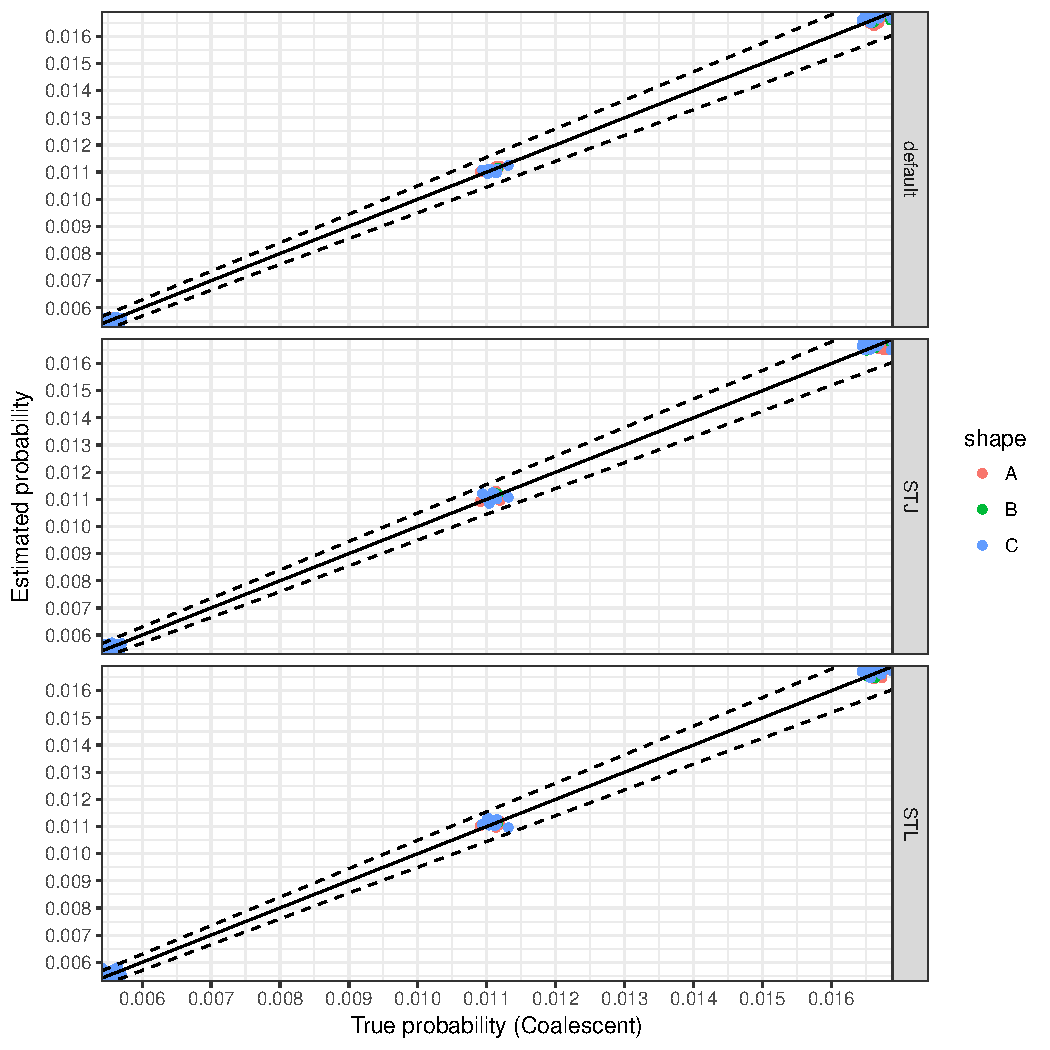
\includegraphics[width=\textwidth, height = 15cm]{\dir/figs/TreeProbabilities_5taxa.pdf}
\caption[Tree probabilities obtained by sampling from the prior with each transition kernel.]{\textbf{Tree probabilities obtained by sampling from the prior with each transition kernel}.
For each tree kernel, we present the estimated probabilities for each of the $105$ possible trees on $5$ taxa from a sample of $M = 1, 000, 000$  trees.
On the x-axis, we present the true probabilities, computed from a sample of $K = 100, 000$ trees from the coalescent prior by direct simulation.
For comparison, probabilities estimated using the default mix of kernels in BEAST v.1.8.4 are provided in the top panel.
Solid line shows $x=y$ and the dashed lines show $5\%$ limits.
Colours show the three possible tree shapes for $5$ taxa.
}
\label{fig:treeP}
\end{figure}
%%%
\begin{figure}[!ht]
\centering
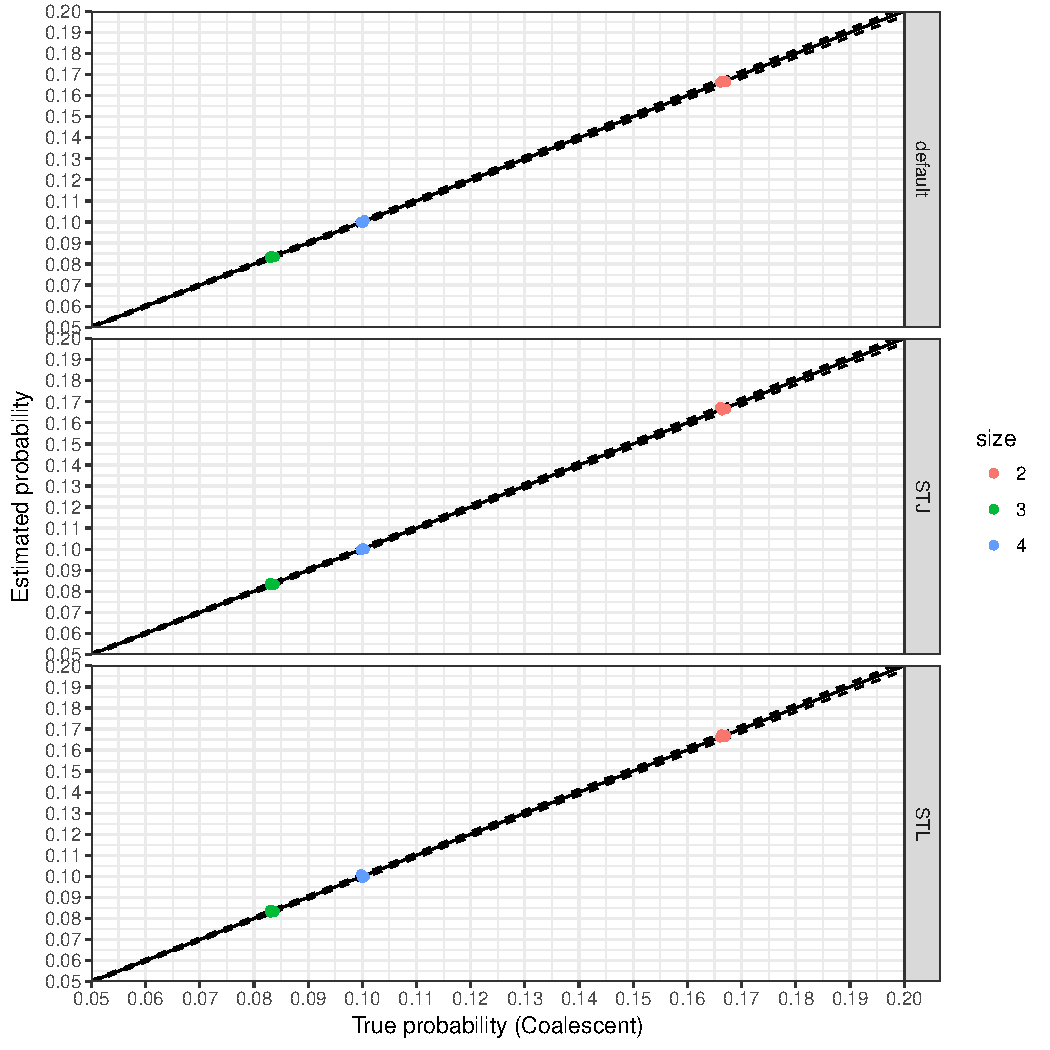
\includegraphics[width=\textwidth, height = 15cm]{\dir/figs/CladeFrequencies_5taxa.pdf}
\caption[Clade probabilities obtained by sampling from the prior with each transition kernel.]{\textbf{Clade probabilities obtained by sampling from the prior with each transition kernel}.
We used the same sample of $1$ million trees to compute clade frequencies to compute the clade frequencies.
On the x-axis, we present the true clade probabilities, computed from a the same sample from the prior as before.
Probabilities estimated using the default mix of kernels in BEAST v.1.8.4 are again provided in the top panel.
Solid line shows $x=y$ and the dashed lines show $1\%$ limits.
Colours show the three possible clade sizes for $5$ taxa (excluding singletons and the set of all leaves/tips).
}
\label{fig:cladeP}
\end{figure}
%%%
\begin{figure}
\begin{center}
 \subfigure[\textbf{Coalescent simulation}]{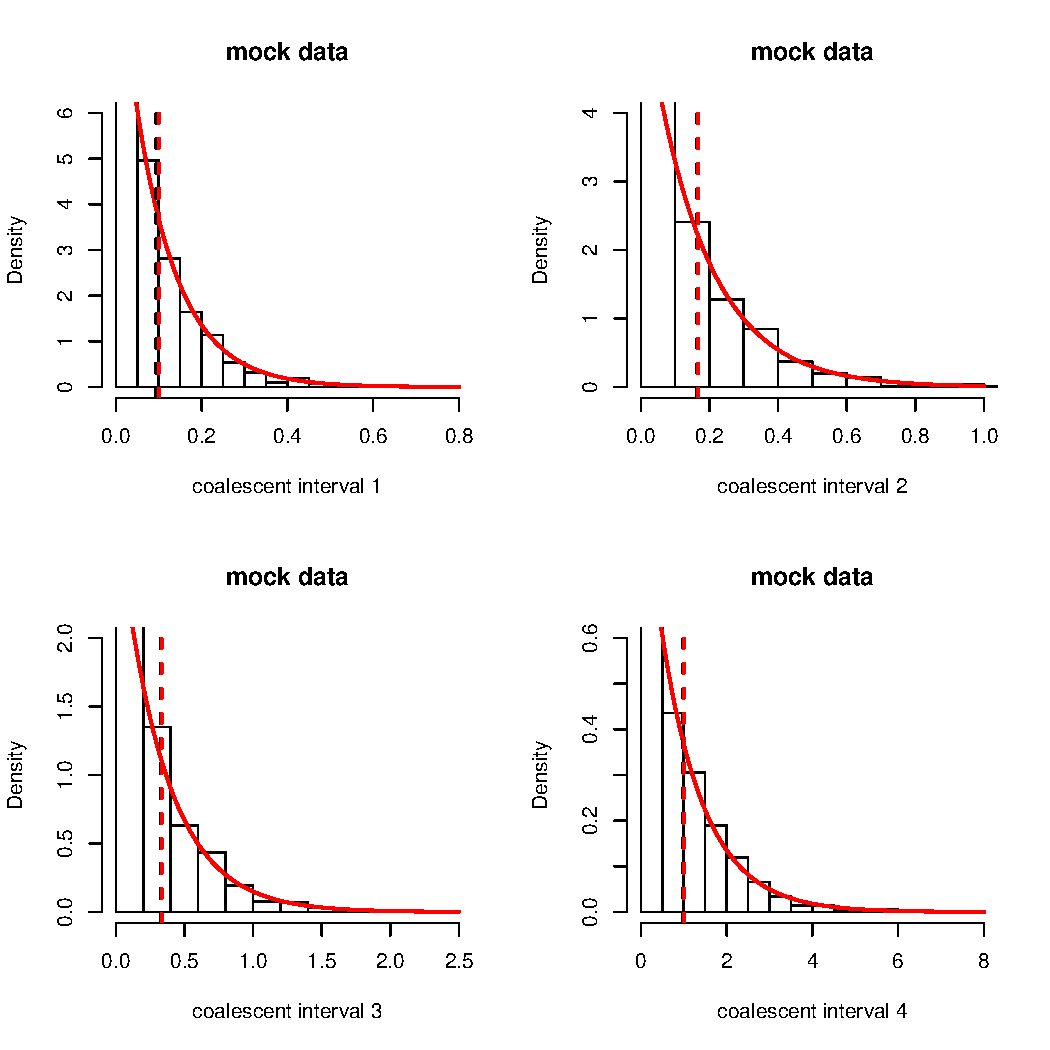
\includegraphics[scale=0.45]{\dir/figs/coalInts_coalSim.pdf}}\\
\subfigure[\textbf{Default operators}]{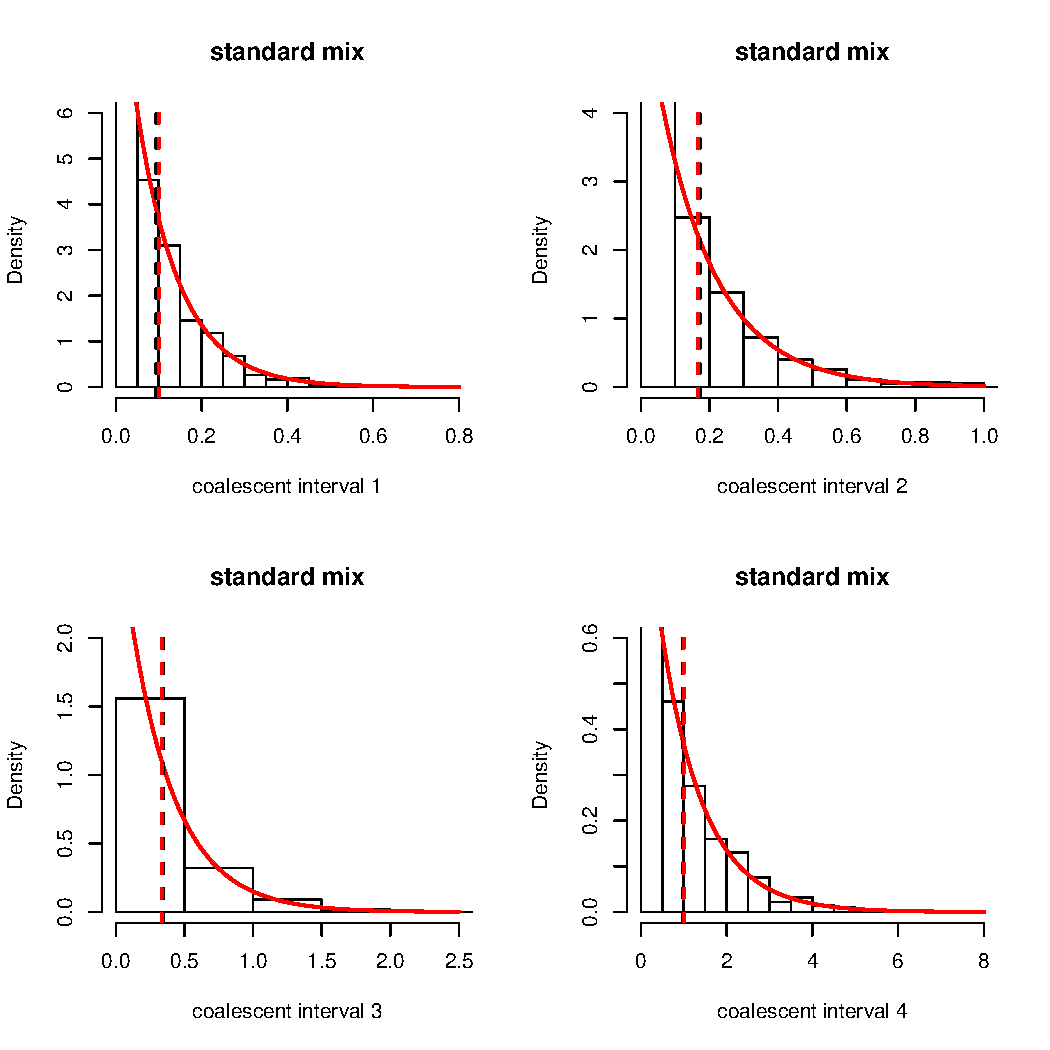
\includegraphics[scale=0.45]{\dir/figs/coalInts_standard_mix.pdf}} \\
\subfigure[\textbf{SubtreeJump (gFNPR)}]{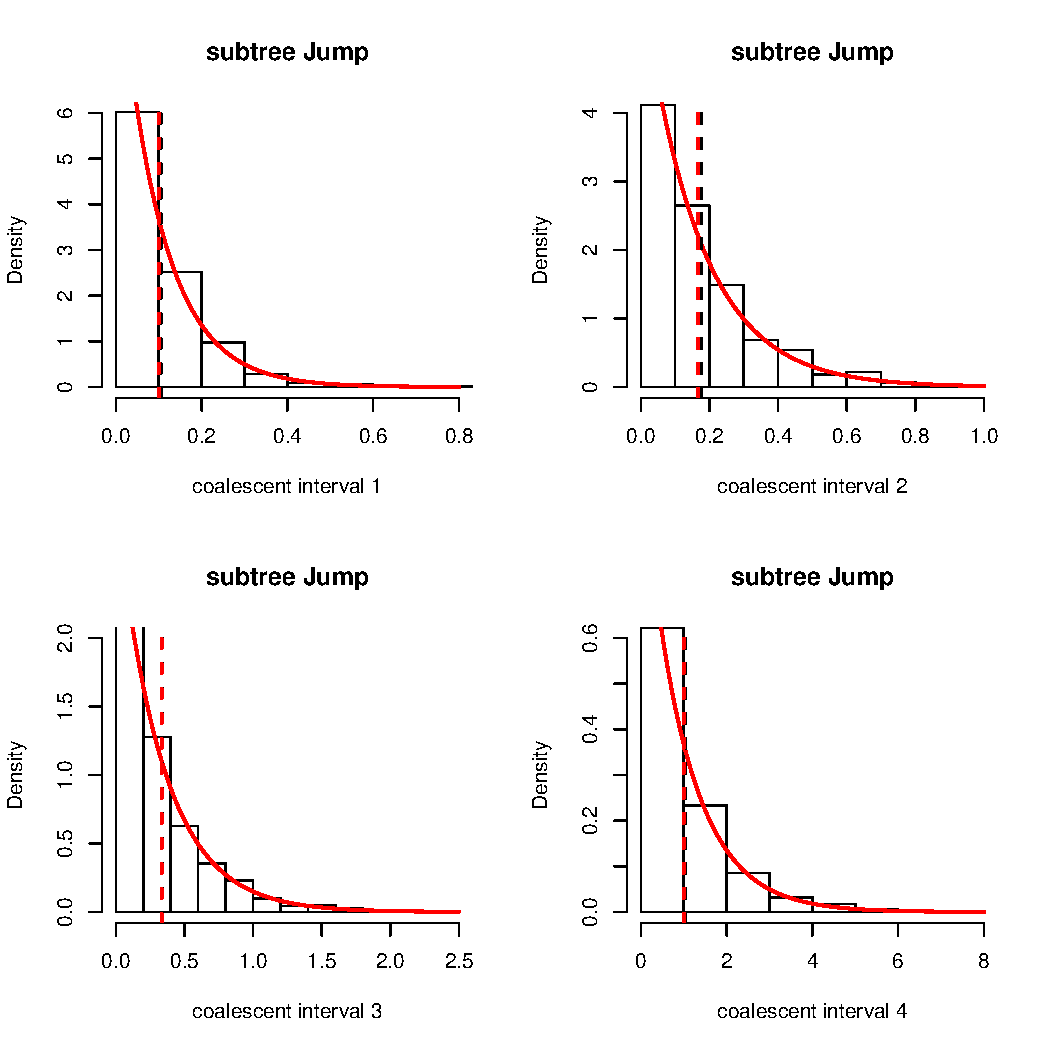
\includegraphics[scale=0.45]{\dir/figs/coalInts_SubTreeJump.pdf}}\\
\subfigure[\textbf{SubTreeLeap}]{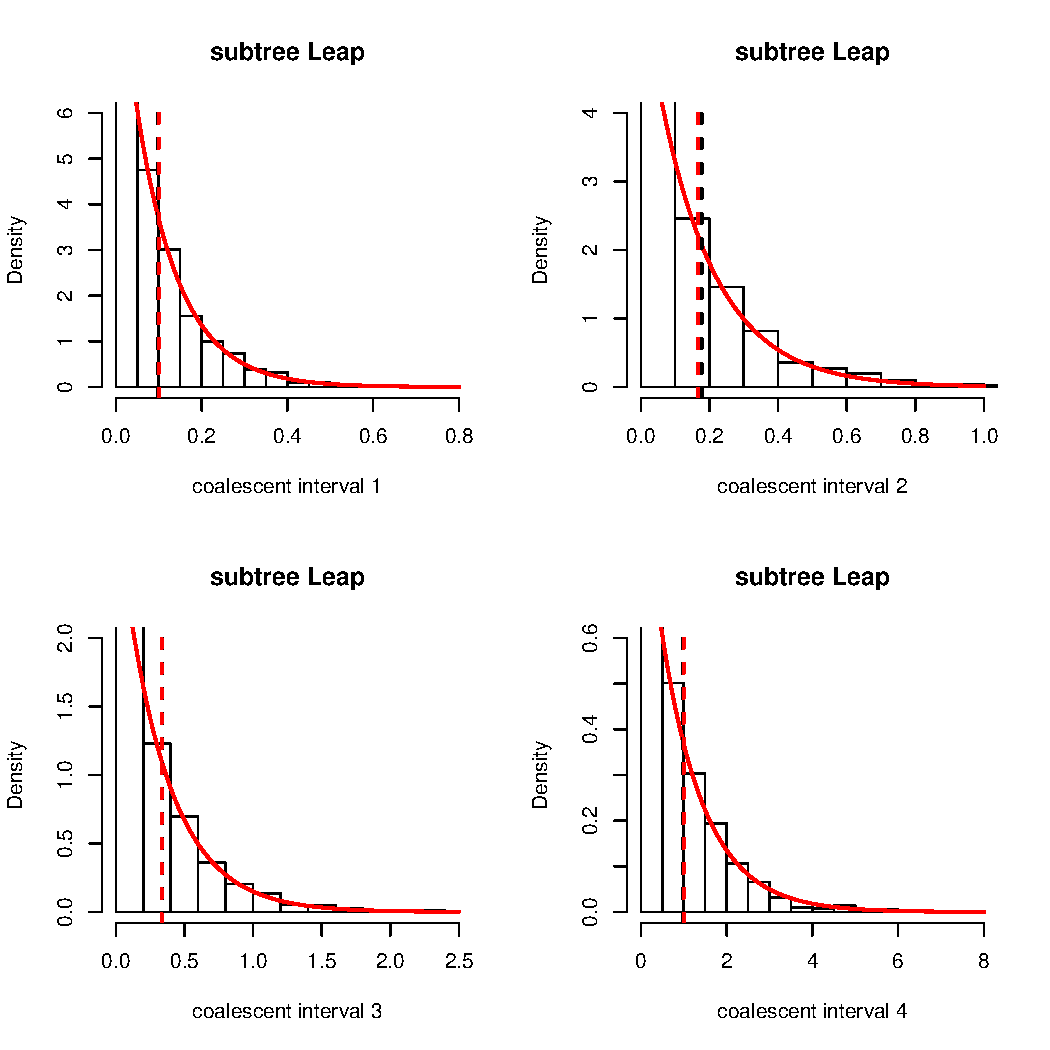
\includegraphics[scale=0.45]{\dir/figs/coalInts_SubTreeLeap.pdf}}
\end{center}
\caption[Coalescent interval distributions obtained by direct simulation, the default (standard) mix of operators in BEAST and our two new kernels.]{\textbf{Coalescent interval distributions obtained by direct simulation, the default (standard) mix of operators in BEAST and our two new kernels}.
We show the distributions of the four coalescent intervals for $n = 5$ and $N_e = 1000$  obtained by (a) direct simulation from the coalescent process, (b) sampling with the default mix of operators (kernels), (c) SubTreeJump and (d) SubTreeLeap.
Red and black vertical dashed lines show the theoretical and estimated means, respectively, and the solid red line shows the theoretical density. 
To be able to sample with SubtreeJump, we need to combine it with branch length transition kernels, whilst SubTreeLeap can sample on its own.
}
\label{fig:coalIntervals}
\end{figure}
%%%
\begin{figure}[!ht]
\centering
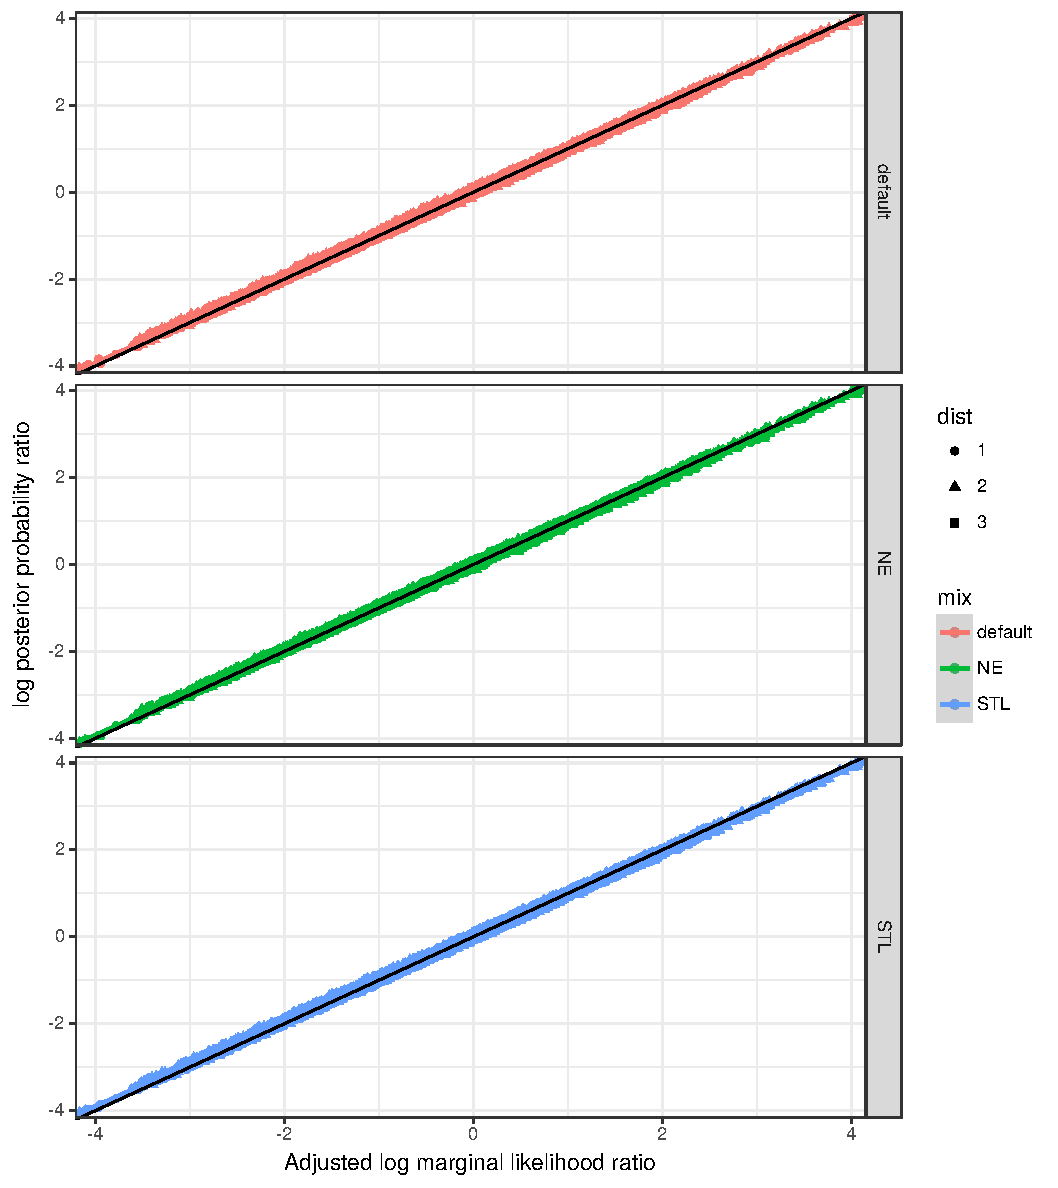
\includegraphics[width=\textwidth, height = 15cm]{\dir/figs/NE_ratioP_vs_ratioMargLike_40L_1Biter.pdf}
\caption[Log posterior probabilities versus marginal (log) likelihoods.]{\textbf{Log posterior probabilities versus marginal (log) likelihoods}.
We plot $\log P_i - \log P_j$ against $(\log l_i - \log l_j) + (\log \pi(T_i) - \log\pi(T_j)$ for the default mix and SubTreeLeap.
Points are coloured according to their rspr distance to the true tree.
Notice that distance zero means the true tree, used to be simulate the data.
}
\label{fig:logP}
\end{figure}
%%%
%%% 
\begin{figure}[!ht]
\centering
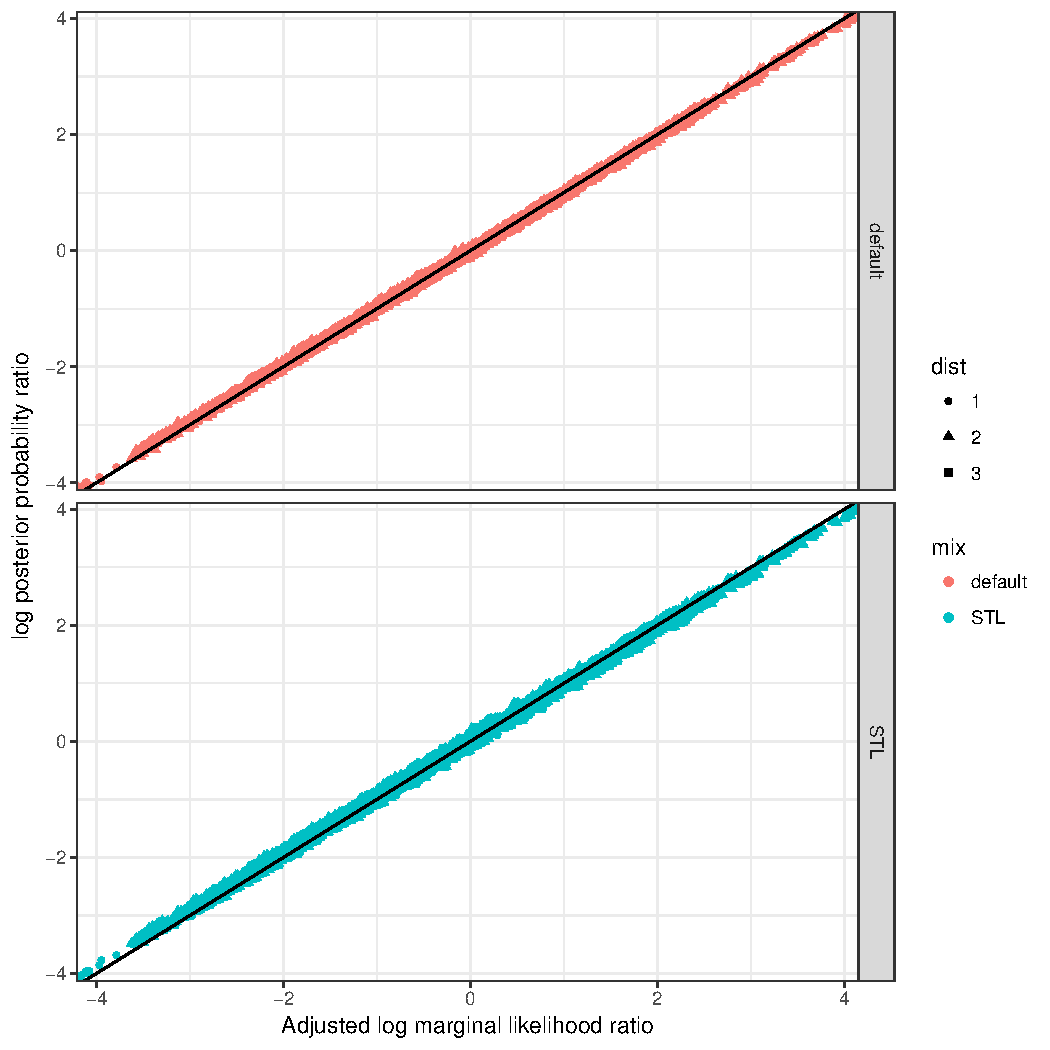
\includegraphics[width=\textwidth, height = 15cm]{\dir/figs/ratioP_vs_ratioMargLike_40L_1Biter.pdf}
\caption[Ratios of posterior probabilities of the trees against the ratio of their marginal likelihoods.]{\textbf{Ratios of posterior probabilities of the trees against the ratio of their marginal likelihoods.}
In this figure we show the (log) ratios as proposed by~\cite{Hoehna2008}.
All computations as in Figure~\ref{fig:logP}.
Solid black line shows $x = y$.
Point shapes depict the distance between the pair of trees.
}
\label{fig:ratios}
\end{figure}  
